\section{Learning to Learn in MARL}\label{sec:approach}   
This section explores learning policies that can adapt quickly to non-stationarity in the policies of other agents in the environment.      
To achieve this, we leverage meta-learning and devise a new \textit{meta-multiagent policy gradient theorem} that exploits the inherent sequential dependencies of MARL discussed in the previous section. 
Specifically, our meta-agent addresses this non-stationarity by considering its current policy's impact on its own adapted policies while actively influencing the future policies of other agents as well by inducing changes to the distribution of trajectories.
In this section, we first outline the meta-optimization objective of MARL and then derive our policy gradient theorem to optimize this objective. 
Finally, we discuss how to interpret our meta-policy gradient theorem with respect to prior work. %which can be seen as a theoretically grounded framework that inherently combines key benefits of previous works by~\citet{alshedivat2018continuous} and~\citet{foerster17lola}.

\subsection{Gradient Based Meta-Optimization in MARL}
We formalize the meta-objective of MARL as optimizing meta-agent $i$'s initial policy parameters $\phi^{i}_{0}$ so that it maximizes the expected adaptation performance over a Markov chain of policies drawn from a stationary initial distribution of policies for the other agents $p(\bm{\phi}^{\bm{-i}}_{\bm{0}})$:
\begin{gather}
\max_{\phi^{i}_{0}}\mathbb{E}_{p(\bm{\phi}^{\bm{-i}}_{\bm{0}})}\Big[\smallsum_{\ell=0}^{L-1}V^{i}_{\bm{\phi}_{\bm{0}:\bm{\ell+1}}}(s_0,\phi^{i}_{0})\Big],\label{eqn:meta-value-function}\\
V^{i}_{\bm{\phi}_{\bm{0:\ell+1}}}\!(s_0,\!\phi^{i}_{0})\!=\!\mathbb{E}_{p(\tau_{\bm{\phi}_{\bm{0:\ell}}}\!|\bm{\phi}_{\bm{0:\ell}})}\!\Big[\mathbb{E}_{p(\tau_{\bm{\phi}_{\bm{\ell+1}}}\!|\bm{\phi}_{\bm{\ell+1}})}\!\big[G^{i}\!(\tau_{\!\bm{\phi}_{\bm{\ell+1}}})\big]\!\Big]\nonumber\!,
\end{gather}
where $\tau_{\bm{\phi}_{\bm{0:\ell}}}\!=\!\{\tau_{\bm{\phi}_{\bm{0}}},\sdots,\tau_{\bm{\phi}_{\bm{\ell}}}\}$ and $V^{i}_{\bm{\phi}_{\bm{0:\ell+1}}}(s_0,\phi^{i}_{0})$ denotes the meta-value function.
This meta-value function generalizes the notion of each agent's primitive value function for the current set of policies $V^{i}_{\bm{\phi}_{\bm{0}}}(s_{0})$ over the length of the Markov chain of policies. 
In this work, we assume that the Markov chain of policies is governed by a policy gradient update function that corresponds to what is generally referred to as the inner-loop optimization in the literature:
\begin{align}\label{eqn:inner-loop}
\begin{split}
\phi^{i}_{\ell+1}\!=& U^{i}(\tau_{\bm{\phi}_{\bm{\ell}}},\phi^{i}_{\ell})\!:=\!\phi^{i}_{\ell}\!+\!\alpha^i\nabla_{\!\phi^{i}_{\ell}}\mathbb{E}_{p(\tau_{\bm{\phi}_{\bm{\ell}}}|\bm{\phi}_{\bm{\ell}})}\Big[G^{i}(\tau_{\bm{\phi}_{\bm{\ell}}})\Big]\!,\\
\bm{\phi}^{\bm{-i}}_{\!\bm{\ell+1}}\!\!=& U^{\!-i}\!(\tau_{\!\bm{\phi}_{\bm{\ell}}},\!\phi^{\!-i}_{\ell})\!\!:=\!\bm{\phi}^{\!\bm{-i}}_{\bm{\ell}}\!\!+\!\hspace{-0.1em}\bm{\alpha}^{\!\bm{-i}}\nabla_{\!\!\!\bm{\phi}^{\!\bm{-i}}_{\bm{\ell}}}\mathbb{E}_{p(\tau_{\bm{\phi}_{\bm{\ell}}}\!|\bm{\phi}_{\bm{\ell}})}\!\hspace{-0.1em}\Big[\!\bm{G}^{\bm{-i}}\!(\tau_{\bm{\phi}_{\bm{\ell}}})\!\Big]\!,
\raisetag{38pt}
\end{split}
\end{align}
where $\alpha^i$ and $\bm{\alpha}^{\bm{-i}}$ denote the learning rates.

\subsection{The Meta-Multiagent Policy Gradient Theorem}\label{sec:meta-mapg-theorem}
% Intuitively, if we optimize the meta-value function in~\cref{eqn:meta-value-function}, we are searching for initial parameters $\phi^{i}_{0}$ such that successive inner-loop optimization steps with~\Cref{eqn:inner-loop} results in adapted parameters $\phi^{i}_{\ell+1}$ that can perform better than the updated policies of other agents with policy parameters $\bm{\phi}^{\bm{-i}}_{\bm{\ell+1}}$ (see~\Cref{fig:graph-meta-mapg}). 
% In deep MARL, a practical way to optimize a value function is by following its gradient. 
% In this section, we consider doing away with the implicit assumption from~\citet{alshedivat2018continuous} discussed in the last subsection that we can ignore the dependence of the future parameters of other agents on $\phi^{i}_{0}$.
A meta-agent needs to account for both its own learning process and the learning processes of other peer agents in the environment to fully address the inherent non-stationarity of MARL. 
We will now demonstrate that our generalized meta-policy gradient includes terms that explicitly account for the effect a meta-agent's current policy will have on its own adapted future policies as well as the future policies of peers interacting with it.

\textbf{Theorem 1.} (Meta-Multiagent Policy Gradient Theorem) \textit{For any stochastic game $\mathcal{M}_{n}$, the gradient of the meta-value function for agent $i$ at state $s_0$ with respect to current policy parameters $\phi_0^i$ evolving in the environment along with other peer agents using initial parameters $\bm{\phi}_{\bm{0}}^{\bm{-i}}$ is:}
\begin{align}\label{eqn:meta-multiagent-policy-gradient}
\begin{split}
&\nabla_{\!\!\phi^{i}_{0}}\!V^{i}_{\!\bm{\phi}_{\bm{0:\ell+1}}}\!(s_0,\!\phi^{i}_{0})\!=\!\mathbb{E}_{p(\tau_{\bm{\phi}_{\bm{0:\ell}}}\!|\bm{\phi}_{\bm{0:\ell}})}\!\Big[\!\mathbb{E}_{p(\tau_{\bm{\phi}_{\bm{\ell+1}}}\!|\bm{\phi}_{\bm{\ell+1}})}\!\big[\!G^{i}(\hspace{-0.1em}\tau_{\hspace{-0.1em}\bm{\phi}_{\bm{\ell+1}}}\hspace{-0.1em})\\
&\;\;\big(\underbrace{\nabla_{\!\!\phi^{i}_{0}}\!\log\!\pi(\tau_{\bm{\phi}_{\bm{0}}}\!|\phi^{i}_{0})}_{\text{Current Policy}}\!+\!\underbrace{\smallsum\nolimits_{\ell'\!=0}^{\ell}\!\!\nabla_{\!\!\phi^{i}_{0}}\!\log\!\pi(\tau_{\bm{\phi}_{\bm{\ell'+1}}}\!|\phi^{i}_{\ell'+1})}_{\text{Own Learning}}+\\
&\;\;\;\underbrace{\smallsum\nolimits_{\ell'\!=0}^{\ell}\!\!\nabla_{\!\!\phi^{i}_{0}}\!\log\!\pi(\tau_{\bm{\phi}_{\bm{\ell'+1}}}\!|\bm{\phi}^{\bm{-i}}_{\bm{\ell'+1}})}_{\text{Peer Learning}}\big)\big]\Big].
\raisetag{63pt}
\end{split}
\end{align}
\textit{Proof.} \hspace{0.2em}See~\cref{sec:proof-meta-multiagent-pg} for a detailed proof.\QEDB

In particular, Meta-MAPG has three primary terms. The first term corresponds to the standard policy gradient with respect to the current policy parameters used during the initial trajectory. Meanwhile, the second term $\nabla_{\phi^{i}_{0}}\log\pi(\tau_{\bm{\phi}_{\bm{\ell'+1}}}|\phi^{i}_{\ell'+1})$ explicitly differentiates through $\log\pi(\tau_{\bm{\phi}_{\bm{\ell'+1}}}|\phi^{i}_{\ell'+1})$ with respect to $\phi^{i}_{0}.$ 
This enables a meta-agent to model its own learning dynamics and account for the impact of $\phi^{i}_{0}$ on its eventual adapted parameters $\phi^{i}_{\ell'+1}$. 
% As such, we can see how this term would be quite useful in improving adaptation across a Markov chain of policies. Indeed, it directly accounts for an agent's own learning process during meta-optimization in order to improve future performance. 
By contrast, the last term $\nabla_{\phi^{i}_{0}}\log\pi(\tau_{\bm{\phi}_{\bm{\ell'+1}}}|\bm{\phi}^{\bm{-i}}_{\bm{\ell'+1}})$ aims to additionally compute gradients through the sequential dependency between the meta-agent's initial policy $\phi^{i}_{0}$ and the future policies of other agents in the environment $\bm{\phi}^{\bm{-i}}_{\bm{1:\ell+1}}$.
As a result, the peer learning term enables a meta-agent to learn to change $\tau_{\bm{\phi}_{\bm{0}}}$ in a way that influences the future policies of other agents and improves its adaptation performance over the Markov chain of policies. 

Interestingly, the peer learning term that naturally arises when taking the gradient in Meta-MAPG is similar to a term previously considered in the literature by \citet{foerster17lola}. 
However, for the Learning with Opponent Learning Awareness (LOLA) approach \citep{foerster17lola}, this term was derived in an alternate way following a first order Taylor approximation with respect to the value function. Moreover, the own learning term previously appeared in the derivation of Meta-PG \citep{alshedivat2018continuous}.
Indeed, it is quite surprising to see how taking a principled policy gradient while leveraging a more general set of assumptions leads to a unification of the benefits of key prior work \citep{alshedivat2018continuous,foerster17lola} on adjusting to the learning behavior of other agents in MARL. 

\subsection{Connection to the Meta-Policy Gradient Theorem}\label{sec:meta-pg-theorem}
The framework of~\citet{alshedivat2018continuous} derived the meta-policy gradient theorem for optimizing a setup like this. 
However, it is important to note that they derived this gradient while making the implicit assumption to ignore the sequential dependence of the future parameters of other agents on $\phi^{i}_{0}$, resulting in the missing peer learning term:
\begin{align}\label{eqn:meta-policy-gradient}
\begin{split}
&\nabla_{\!\!\phi^{i}_{0}}\!V^{i}_{\!\bm{\phi}_{\bm{0:\ell+1}}}\!(s_0,\!\phi^{i}_{0})\!=\!\mathbb{E}_{p(\tau_{\bm{\phi}_{\bm{0:\ell}}}\!|\bm{\phi}_{\bm{0:\ell}})}\!\Big[\!\mathbb{E}_{p(\tau_{\bm{\phi}_{\bm{\ell+1}}}\!|\bm{\phi}_{\bm{\ell+1}})}\!\big[\!G^{i}(\hspace{-0.1em}\tau_{\hspace{-0.1em}\bm{\phi}_{\bm{\ell+1}}}\hspace{-0.1em})\\
&\;\;\big(\underbrace{\nabla_{\!\!\phi^{i}_{0}}\!\log\!\pi(\tau_{\bm{\phi}_{\bm{0}}}\!|\phi^{i}_{0})}_{\text{Current Policy}}\!+\!\underbrace{\smallsum\nolimits_{\ell'\!=0}^{\ell}\!\!\nabla_{\!\!\phi^{i}_{0}}\!\log\!\pi(\tau_{\bm{\phi}_{\bm{\ell'+1}}}\!|\phi^{i}_{\ell'+1})}_{\text{Own Learning}}\big)\big]\Big]\!.
\raisetag{30pt}
\end{split}
\end{align}
\textbf{Remark 1.} \textit{
Meta-PG can be considered as a special case of Meta-MAPG when assuming that other agents' learning in the environment is independent of the meta-agent's behavior.}

\textit{Proof.} \hspace{0.2em}See~\cref{sec:proof-meta-pg} for a corollary.\QEDB

Specifically, Meta-PG treats other agents as if they are external factors whose learning it cannot affect.
For example, a meta-agent in~\citet{alshedivat2018continuous} competes against an opponent that has been pre-trained with self-play. The next agent after the current interaction is then loaded as the same opponent with one more step of training with self-play. 
As a result of this contrived setup, the opponent's policy update is based on data collected without a meta-agent presented in the environment and Meta-PG can get away with assuming that the peer's learning process is not a function of a meta-agent's behavior.
However, we note that this assumption does not hold in practice for the general multi-agent learning settings we explore in this work. 
As highlighted in~\cref{sec:background-non-stationarity}, every agent's policy jointly affects the environment's transition and reward functions, resulting in the inherent sequential dependencies of MARL. Therefore, a meta-agent's behavior can affect the future policies of its peers, and these cannot be considered as external factors.
% the assumption is not general and can be the main cause of the lack of adaptation performance.
% As shown by the ... markov chain in Section X, because all agents' policies jointly affect the environment's transition and reward functions, ... sequential dependiences. ... thus they affect one another and cannot be considered as an external factor.

% the opponent agent is pre-trained via self-play~\citep{bansal2018emergent} and its policy is saved at each iteration in~\citet{alshedivat2018continuous}.
% Then, a meta-agent competes against the increasing snapshot version of the pre-trained opponent throughout the Markov chain.
% a meta-agent competes against the pre-trained opponent saved at each iteration, and  opponent's policy version throughout the Markov chain.
% the opponent policy version increased throughout the Markov chain to adapt to increasingly more competent versions of the opponent.
% We snapshot and save versions of the pre-trained policies at each iteration. This lets us train other agents to play against versions of the pre-trained opponents at various stages of mastery
% The agents have to keep adapting to increasingly more competent versions of the opponent
% Next, we run iterated games between our trained agents that use different adaptation algorithms versus policy snapshots of the pre-trained opponents. Crucially, the policy version of the opponent keeps increasing from round to round as if it was training via self-play. 
% For example, in the competitive environment, the opponent interacting with a meta-agent was pre-trained and different opponent version was loaded for a meta-agent's adaptation. 

\noindent\header{Probabilistic model perspective.}
Probabilistic models for Meta-PG and Meta-MAPG are depicted in~\cref{fig:graph-meta-mapg}.
As shown by the own learning gradient direction, a meta-agent $i$ optimizes $\phi^{i}_{0}$ by accounting for the impact of $\phi^{i}_{0}$ on its updated parameters $\bm{\phi}^{\bm{i}}_{\bm{1:\ell+1}}$ and adaptation performance $G^{i}(\tau_{\bm{\phi}_{\bm{\ell+1}}})$.
However,  Meta-PG considers the other agents as external factors that cannot be influenced by the meta-agent, as indicated by the absence of the sequential dependence between $\tau_{\bm{\phi}_{\bm{0:\ell}}}$ and $\bm{\phi}^{\bm{-i}}_{\bm{1:\ell+1}}$ in~\Cref{fig:graph-meta-mapg}. 
As a result, the meta-agent loses an opportunity to influence the future policies of other agents and further improve its adaptation performance, which can cause undesirable learning failures as highlighted by the following motivating example.
% as other agents are learning. 
% By contrast, the peer learning term in Theorem 1 aims to additionally compute gradients through the sequential dependency between the agent's initial policy $\phi^{i}_{0}$ and the future policies of other agents in the environment $\bm{\phi}^{\bm{-i}}_{\bm{1:\ell+1}}$ so that it can learn to change $\tau_{\bm{\phi}_{\bm{0}}}$ in a way that maximizes performance over the Markov chain of policies.

%%%%%%%%%%%%%%%%%%%%%%%%%%%%%%%%
\begin{figure}[t]
    \centering
    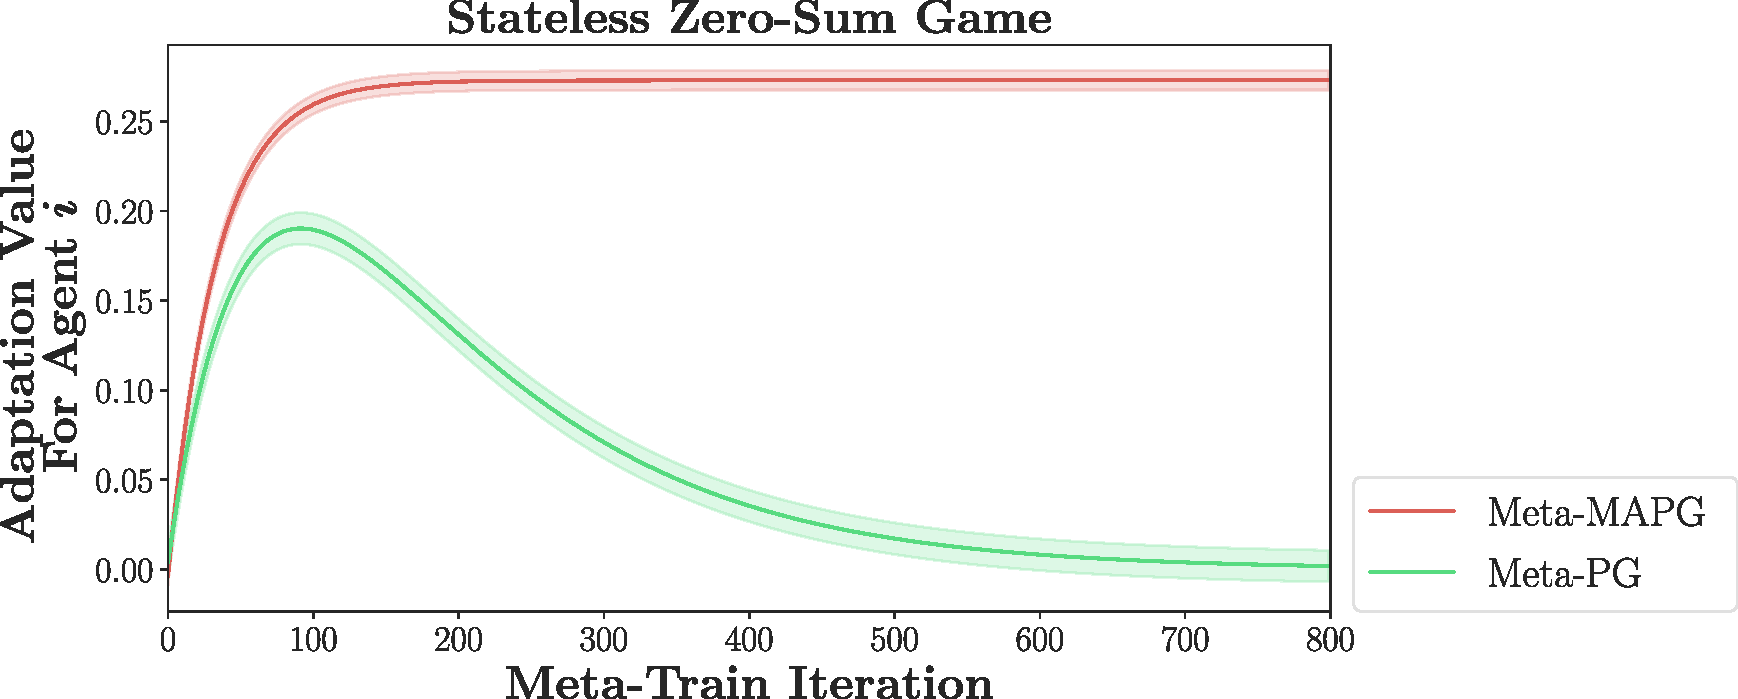
\includegraphics[height=2.9cm]{figs/toy.pdf}
    \vspace{-0.3cm}
    \caption{Meta-training result in the stateless zero-sum game when training a meta-agent $i$ with either Meta-PG~\citep{alshedivat2018continuous} or Meta-MAPG. Meta-MAPG achieves better adaptation than Meta-PG thanks to the peer learning gradient. Mean and 95\% confidence interval computed for 200 random samples are shown.
    }
    \label{fig:toy-example}
    \vskip-0.2in
\end{figure}
%%%%%%%%%%%%%%%%%%%%%%%%%%%%%%%%

\textbf{Example 1.} \textit{Failure to consider our influence on the learning of other agents can result in biased and sometimes even counterproductive optimization.}

For example, consider a stateless zero-sum game played between two agents based off the one shown by \citet{letcher2018stable}.
A meta-agent $i$ and an opponent $j$ maximize simple value functions $V^{i}_{\bm{\phi}_{\bm{\ell}}}\!=\!\phi^{i}_{\ell}\phi^{j}_{\ell}$ and $V^{j}_{\bm{\phi}_{\bm{\ell}}}\!=\!-\phi^{i}_{\ell}\phi^{j}_{\ell}$ respectively, where $\phi^{i}_{\ell},\phi^{j}_{\ell}\!\in\!\mathbb{R}$. 
We assume a maximum Markov chain length $L$ of 1 and focus on meta-agent $i$'s adaptation performance $V^{i}_{\bm{\phi}_{\bm{1}}}$. 
Given an opponent's initial policy parameters randomly sampled from $p(\bm{\phi}^{\bm{-i}}_{\bm{0}})$, we compare training a meta-agent $i$ with either Meta-PG or Meta-MAPG.
As~\cref{fig:toy-example} shows, Meta-PG performs biased updates that actually make its performance worse over the course of meta-training. 
% The cause of the failure in this example is due to the stationary assumption that each agent assumes its opponent has the same behavior in the future~\citep{letcher2018stable}.
In contrast, by considering the opponent's learning process, Meta-MAPG corrects for this bias, displaying smooth convergence to a winning strategy.
%As such, it is important to consider others' learning process as highlighted by this example. -- probably redundant
See~\cref{sec:details-stateless-zero-sum} for more details, including the meta-gradient derivation.

\subsection{Algorithm}
% \noindent\paragraph{Algorithm.}
We provide pseudo-code for Meta-MAPG in~\cref{alg:meta-train} for meta-training and~\cref{alg:meta-test} for meta-testing in~\Cref{sec:meta-mapg-algorithm}.
Note that Meta-MAPG is centralized during meta-training as it requires the policy parameters of other agents to compute the peer learning gradient. 
For settings where a meta-agent cannot access the policy parameters of other agents during meta-training, we provide a decentralized meta-training algorithm with opponent modeling, motivated by the approach used in~\citet{foerster17lola}, in~\cref{sec:opponent-modelling} that computes the peer learning gradient while leveraging only an approximation of the parameters of peer agents.
Once meta-trained in either case, the adaptation to new agents during meta-testing is purely decentralized such that the meta-agent can decide how to shape other agents with its own observations and rewards alone. 